\chapter{Redes Metabólicas}
 
\indent Neste capítulo serão descritos os conceitos básicos da biologia molecular, metabolismo e bancos de dados específicos para redes metabólicas. A primeira seção detalha a origem das principais estruturas que promovem o metabolismo tais como DNA e enzima, enquanto que a segunda seção descreve de fato como ocorre o processo. Por fim, a última seção apresenta os principais bancos de dados em grafo voltados para redes metabólicas: \textit{KEGG}, \textit{MetaCyc} e \textit{Reactome}.


%% ================================================================================================================== %%


\section{Conceitos Básicos de Biologia Molecular}


\subsection{Ácidos Nucléicos} \label{aceidosNucleicos}

\indent Os ácidos nucleicos são biomoléculas responsáveis pelo armazenamento, transmissão e tradução das informações genéticas dos seres vivos. Isto é possível devido ao processo de síntese de proteínas que permite, assim, a base da herança biológica.Os acidos nucléicos são polímero, macromoléculas formadas por estruturas menores chamadas monômeros, que nesse caso são nucleotídeos. Nucleotídeos são compostos de três elementos: um radical fosfato (HPO$_{4}$), uma pentose, ou seja, um monossacarídeo formado por cinco átomos de carbono, e uma base nitrogenada. Existem cinco tipos de bases nitrogenadas que podem compor um nucleotídeo: Adenina(A), Timina(T), Citosina(C), Guanina(G) e Uracila(U). \\

\begin{figure}[h]
    \centering
    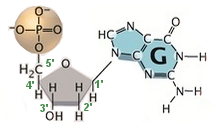
\includegraphics[width=0.5\textwidth]{nucleotideo.png}
    \caption{imagem de um nucleotídeo e das bases nitrogenadas. Mostrar backbone da pentose 1'...5'. Adaptado de : \cite{dnadiscovery08}. }
    \label{fig:Nucleotideo}
\end{figure} 

\indent Na figura \ref{fig:Nucleotideo}, observa-se que no \textit{backbone} do nucleotídeo existe uma numeração de 1' à 5', que representam os carbonos presentes na pentose. Para a criação de uma fita de ácido nucleico, no processo de polimerização formar-se uma ligação fosfodiéster entre o carbono da posição 5' do \textit{backbone} de um nucleotídeos e o carbono de posição 3' do \textit{backbone} de outro \cite{setubal97}. Por definição o sentido da leitura de uma fita de ácido nucleido é 5' $\rightarrow$ 3', o que é deve ser levado em consideração ao se fazer interpretação de dados do material genético.

\indent Dois tipos de ácidos nucleicos são encontrados nos seres vivos: ácido desoxirribonucleico (DNA ou ADN) e ácido ribonucleico (RNA ou ARN). Eles diferenciam-se tanto na estrutura do \textit{backbone} e nas bases nitrogenadas, quanto em suas funções. Os DNAs são as biomoléculas que armazenam as informações referentes ao funcionamento de todas as células dos seres vivos de maneira específica: sequências de pares de bases nitrogenadas. Nesse sentido, além de haver a ligação fosfodiéster entre os nucleotídeos, cada um também se liga a partir de suas bases nitrogenadas, formando assim um eixo helicoidal tridimensional chamada de dupla hélice \cite{setubal97}. Esta estrutura foi descoberta em 1953, pelo biólogo James Watson e pelo físico Francis Crick \cite{dnadiscovery08}, porém os ácidos nucleicos já eram estudado desde 1869 na Suíça pelo químico-fisiológico Friedrich Miescher.

\indent Em relação à estrutura dos monômeros do DNA, o \textit{backbone} dos nucleotídeos é uma desoxirribose, indicada na figura \ref{fig:EstruturasDoDNA}. Para a formação da dupla hélice, os pares são feitos com uma base nitrogenada do grupo de purinas, composto orgânico que possui um anel duplo de carbono, e outra base do grupo de pirimidinas, composto orgânico que possui um anel simples de carbono. No caso do DNA, somente quatro das cinco bases são empregadas: as purinas Adenina(A) e Guanina(G), que se ligam com as pirimidinas Timina(T) e Citosina(C) respectivamente. Desta forma, A e T são bases complementares, assim como G e C. Uma fita de DNA pode conter centenas de milhões de nucleotídeos.

\indent A representação do DNA, seja nos livros ou computacionalmente, é dada por um par em paralelo de strings de letras A, T, G e C. Como explicado no início dessa seção, o sentido padrão da leitura de uma fita é de 5' $\rightarrow$ 3', mas no caso do DNA, as hélices são dispostas de maneira antiparalela, ou seja, uma é lida de 5' $\rightarrow$ 3' e a outra, de 3' $\rightarrow$ 5'. Observa-se que a partir de uma hélice, pode-se inferir a sequência de sua hélice complementar. Seja, por exemplo, uma hélice H1 igual a AGTAAGC; então H2 em seu sentido oposto é H2' igual a TCATTCG, e no sentido regular, igual a GCTTACT. A figura \ref{fig:EstruturasDoDNA} apresenta a estrutura do DNA como explicada nesta seção.

\begin{figure}[h]
    \centering
    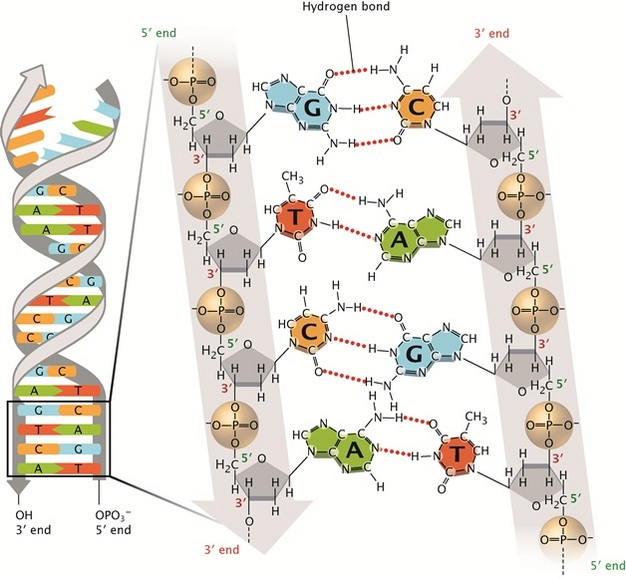
\includegraphics[width=0.7\textwidth]{dnaEstrutura.jpg}
    \caption{Adaptado de : \cite{dnadiscovery08} }
    \label{fig:EstruturasDoDNA}
\end{figure} 

\indent Os RNAs são biomoléculas semelhantes ao DNA, porém contam com três diferenças básicas. A primeira é a estrutura do \textit{backbone} dos nucleotídeos, que é composta por uma ribose ao invés de um desoxirribose. A segunda difereça é em relação às bases nitrogenadas, onde a pirimidina Uracila(U) substitui a Timita(T). Por fim, o RNA é formado por apenas uma hélice tridimensional.

\indent Existem três tipos de RNAs presentes no citoplasma - espaço entre a membrama plasmática e o núcleo da célula. 
Cada um possui funções específicas que serão detalhadas na seção \ref{sinteseDeProteina}. Em suma, O RNA mensageiro (mRNA) é responsável pela transferência de informação do DNA para o RNA ribossômico (rRNA), que por sua vez irá desanexar a proteína do RNA transportador (tRNA) combinando-o com o rRNA, executando assim, a síntese de proteína.



%% ================================================================================================================== %%

\subsection{Síntese de Proteína} \label{sinteseDeProteina}

\indent As proteínas são biomoléculas com diversas responsabilidades no corpo dos seres vivos. Se fizerem parte do no grupo de proteínas fibrosas, como o colágeno, irão compor a estrutura do corpo e para isso precisam ser resistentes e insolúveis em água. Caso estejam no grupo de proteínas globulares, como a hemoglobina, realizarão processos dinâmico pelo corpo tais como transportações e cataliações \cite{profangela11}.  Cada tarefa é realizada por um proteína com uma estrutura específica e otimizada pra tal.

\indent Assim como os ácidos nucleicos, as proteínas são polímeros, macromoléculas cujos monômeros são aminoácidos. Aminoácidos são moléculas que possuem cinco componentes: amina (NH$_{2}$), carbono (C), hidrogênio (H), ácido carboxílico (COOH) e uma cadeia lateral que funciona como identificador de cada um dos 20 tipos de aminoácidos presentes nos seres vivos. A maneira como eles são criados será explicada com mais detalhes mais à frente, pois envolve um processo complexo de síntese de proteína executado pelo ribossomo. A ligação, ou polimerização, de dois aminoácidos é feita unindo a amida de um com o ácido carboxílico do outro, liberando uma molécula de água (H$_{2}$O) e formando uma cadeia chamada de dipeptídeo. Como houve liberação de água na ligação, o dipeptídeo não é formado por aminoácidos, mas sim resíduos dos mesmos. Nesse sentido, cadeias peptídicas de 100 à 5000 diferentes resíduos aminoácidos, ou cadeia polipeptídicas,  constituem a proteína.

\indent Existem quatro estruturas para caracterização de uma proteína \cite{setubal97}. A mais simples é chamada de estrutura primária e é composta por uma sequência linear de resíduos aminoácidos. A estrutura secundária é tridimensional e estabiliza-se por meio de ligações de hidrogênio na cadeia principal, chamada de \textit{backbone}. Dependendo da disposição dos resíduos de aminoácidos, esta cadeia pode se dar forma de hélice ($\alpha$-Helix) ou em forma de folha ($\beta$-Helix). A estrutura terciária é dada pela união de várias estruturas secundárias e, por fim, a estrutura quaternária é composta de múltiplas estruturas terciárias \cite{drug09}. A figura \ref{fig:EstruturasDaProteina} ilustra os quatro tipos de proteínas descritos.

\begin{figure}[h]
    \centering
    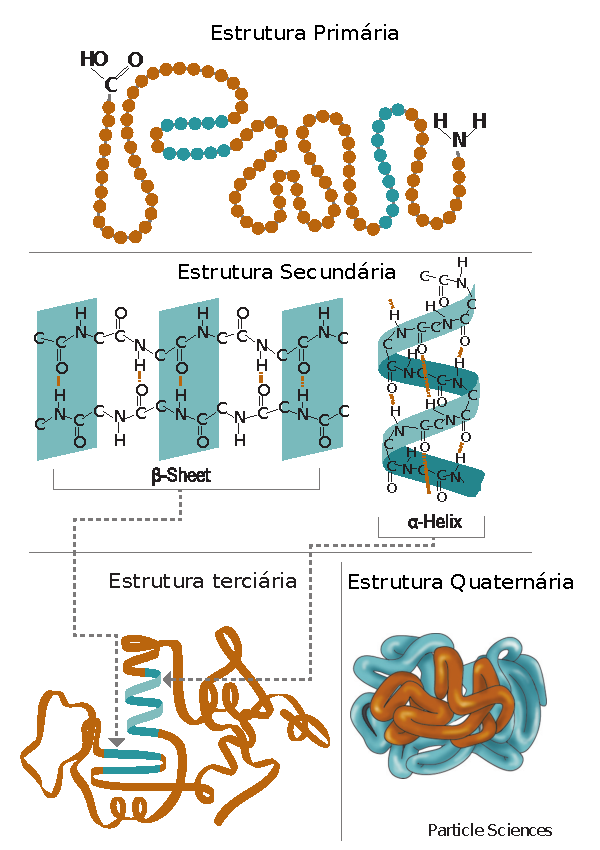
\includegraphics[width=0.6\textwidth]{EstruturasDaProteina.pdf}
    \caption{Adaptado de : \cite{drug09} }
    \label{fig:EstruturasDaProteina}
\end{figure}

% PROCARIÓTAS
\indent A \textbf{transcrição} é o processo de produção de mRNA a partir do DNA e ele ocorre da seguinte forma: O início de cada gene possui um identificador em uma das fitas para indicar o local da codificação e, a partir dali, uma cópia inversa (A, T, C, G são traduzidos para U, A, G, C respectivamente) do mesmo é feita sob forma de molécula de mRNA que, por consequência, obterá a mesma sequência que a cadeia codificadora (a qual não possui o identificador), porém trocando os U's por Ts.

\indent O mRNA deixa, então, o núcleo celular e inicia a \textbf{tradução} no citoplasma. O processo ocorre no interior de uma organela celular chamada de ribossomo, constituído de proteínas e rRNA e cuja função é construir a molécula de proteína a partir de duas entradas, o mRNA e tRNA. A estrutura do tRNA é tal que de um lado se encaixa exatamente um códon (sequência de três nucleotídeos) e no oposto, seu aminoácido correspondente. O processo de tradução se dá da seguinte forma: a medida em que o mRNA passa pelo interior do ribossomo, este atrai quaisquer tRNAs das proximidades cujos códons sejam correspondentes ao da subsequência corrente do mRNA. No momento em que o códon do tRNA se conecta com um dos códons do mRNA, a molécula de proteína em desenvolvimento é liberada e, com o auxílio da catálise de uma enzima, agregada no aminoácido que estava fixado naquele tRNA. Esta fase é finalmente completa quando o mRNA apresenta um códon de parada, pois nenhum tRNA possui correspondência para tal \cite{setubal97}. Uma proteína simples é, então, formada.

%% ================================================================================================================== %%


\section{Conceitos Básicos de Metabolismo}

%D. L. Nelson and M. C. Michael. Princípios de Bioquímica de Lehninger - Ed. Comemorativa 25 Anos. Artmed, São Paulo - SP, 5nd edition, 2010. 4, 5, 6, 7, 8, 11, 13

\indent As reações bioquímicas são alterações químicas que fornecem um ou mais produtos a partir de um ou mais substratos. O conjunto de todas as reações bioquímicas que ocorrem dentro de um organismo vivo é chamado de metabolismo, e ele podem ser dividido em dois subconjuntos: catabolismo, quando ocorre a quebra de moléculas complexas produzindo energia, e anabolismo, quando ocorre a síntese de moléculas complexas, o que requer energia. Geralmente a energia liberada pelas reações catabólicas é usada para impulsionar as reações anabólicas. Uma via metabólica é uma sequência de reações bioquímicas, cujo produto e subtrato são denominados metabólitos, que podem ser catalisados por enzimas, as quais muitas vezes necessitam de compostos químicos chamados de co-fatores para realizarem suas atividades na célula. O conjunto de vias metabólicas de um organismo é chamado de rede metabólica.

\indent Enzimas são proteínas responsáveis por auxiliar a realização de biossíntese (construção) e biodegradação de moléculas no metabolismo com o propósito de catalisar (acelerar) reações bioquímicas. As enzimas possuem um local pré-determinado em formato côncavo chamado de sítio ativo, que comporta um ou mais substratos. Se a enzima comporta apenas um substrato, a estrutura que se forma com o preenchimento do sítio ativo é um complexo enzima-substrato, porém se ela comporta mais de um substrato, a estrutura é chamada de complexo ternário intermediário. %CITAR Biochemical-Pathway, pag 21, 2.4 Enzimes
Quando a atividade catalítica não pode ser realizada apenas pela enzima, co-fatores auxiliam o processo. Eles podem ser coenzimas, associadas momentaneamente às enzima, ou grupos prostéticos, associados firmemente à elas.  %CITAR Biochemical-Pathway, pag 21, 2.4 Enzimes 
Quando duas enzimas possuem a mesma atividade enzimática porém estruturas físicas diferentes são chamadas isoenzimas. %CITAR Biochemical-Pathway, pag 21, 2.4 Enzimes



\subsection{Metabolismo Primário}


\indent No caso em que o metabolismo exerce uma função fundamental no organismo, ele é classificado como metabolismo primário. Mitose e meiose são exemplos de metabolismos primários. Já quando o metabolismo não está relacionado a reprodução, desenvolvimento ou crescimento, ele não é essencial no organismo e, portanto, secundário. Os metabólitos secundários, apesar da aparente insignificância, podem ser antibióticos, por exemplo, e deste modo são bastante aplicados na medicina e na indústria %\cite{waldeyr}.

\subsection{Metabolismo Secundário}




%% ================================================================================================================== %%

\section{Banco de Dados de Redes Metabólicas}

% Dogma central

\indent No início dos anos 50, uma química britânica chamada Rosalind Frankling usou a técnica de difração de raios-X para determinação da estrutura da biomolécula do DNA e concluiu que sua forma era helicoidal. Seu trabalho foi empregado nos experimentos de dois pesquisadores, Francis Crick e James Watson, em um laboratório em Cambridge, na Inglaterra. No mesmo ano, a dupla decifrou a estrutura do DNA: duas longas fitas enroladas uma na outra em espiral para a direita, ligadas por pares de bases complementares, formando o que chamaram de dupla-hélice. Apesar da grande descoberta, isto não era o suficiente para entender como eram produzidas as proteínas, portanto os cientistas mudaram o foco das pesquisas para o RNA, uma vez que sabiam o quanto sua concentração aumentava sempre que as células começavam a produzir proteínas \cite{violinist12}. Em 1958, Crick e Watson anunciaram mais uma descoberta: A partir do DNA, o processo de \textit{transcrição} fornece uma fita de RNA, que por sua vez, a partir do processo de \textit{tradução}, fornecem a proteína. Esta sequência de processos ficou conhecida como Dogma Central da biologia molecular. \\

% Surgimento de bancos de dados (PAM, GenBank)

\indent Conforme o número de sequências de proteínas cresciam, aumentava também a necessidade de criar-se um banco de dados para indexá-las. A físico-química norte-americana Margaret Dayhoff, com colaboração de alguns membros do \textit{National Biomedical Research Foundation} em Washington, foi a primeira a construir um banco de dados com este propósito em um tipo de atlas de proteínas na década de 60. Somente em 1984 esta coleção foi intitulada de \textit{Protein Information Resource} \cite{mount01}. Os dados eram organizados de acordo com o grau de similaridade das sequências, onde o agrupamento das mesmas era dado em forma de árvore filogenética representando famílias e superfamílias de proteínas. Caso a semelhança seja alta, é provável que tenham as mesmas funções bioquímicas e estrutura tridimensional. A partir da árvore gerada, foi possível calcular as mutações que ocorreram nos aminoácidos durante a evolução genética e, então, produzir uma tabela utilizada até hoje, chamada PAM (\textit{percent acept mutation}), que apresenta tais dados. Outro banco de dados de grande porte e bastante utilizado nos dias de hoje é o GenBank, estabelecido em 1982 por Walter Goad e demais colaboradores e, agora, com o patrocínio do \textit{National Center for Biotechnology Information}. Os dois bancos são públicos e continuam crescendo exponencialmente \cite{mount01}.

\section{Banco de Dados NoSQL}

\indent NoSQL

\cite{jing12} 

%https://neo4j.com/docs/developer-manual/current/terminology/

\indent Comparação com SQL \\
%http://dl.acm.org/citation.cfm?id=1721659

\section{Propriedades}

\indent ACID, BASE % ARTIGO Scalable_SQL_and_NoSQL_Data_Stores

\indent Consistency, availability and tolerance of network partition (consistência, disponibilidade e tolerancia de partição de redes) % ARTIGO Survey\_on\_NoSQL\_Database

%
%
% EXEMPLO:
%
%
\section{OrientDB}
%http://orientdb.com/docs/last/
\indent sobre ACID \\
%http://orientdb.com/docs/last/Transactions.html
\indent Modelo CAP \\
%https://github.com/sslavic/orientdb-wiki/blob/master/CAP-Model.md
\indent JAVA API \\
%http://orientdb.com/docs/last/Java-API.html

\subsection{KEGG}

\subsection{BioCyc}

\subsection{Reactome}

